\begin{frame}
	\frametitle{\textbf{1. Problem A: Steady-state Poisson equation}}
    
    Consider a $2$-dimensional unit square $\Omega = (0,1)^d$ and the following problem subjected to homogeneous Dirichlet boundary conditions: 
    \vspace{0.5cm}
    \begin{columns}[c]
    \begin{column}{0.5\textwidth}
    % \vspace*{-\baselineskip}
    \begin{framed}
    Find a scalar $T$ in $\Omega \rightarrow \mathbb{R}$ satisfying:
    \begin{align*}
        -\partial_j \partial_j T =& 10 \ \textrm{ in } \Omega\\
         T =& 0 \ \textrm{ in } \Gamma
    \end{align*}
    \end{framed}
    \end{column}
    \begin{column}{0.4\textwidth}
    \vspace*{-\baselineskip}
    \begin{center}
    	
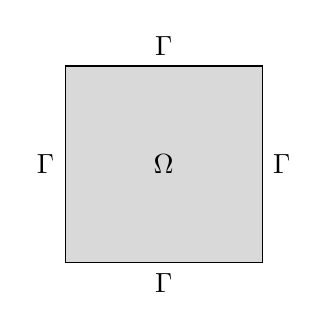
\begin{tikzpicture}[scale=2.5]
	% Draw the shaded square
	\fill[gray!30] (0,0) rectangle (1,1);
	
	% Draw the square outline
	\draw (0,0) rectangle (1,1);
	
	% Label Ω inside the square
	\node at (0.5,0.5) {$\Omega$};
	
	% Label Γ on the boundaries
	\node at (-0.1,0.5) {$\Gamma$};
	\node at (1.1,0.5) {$\Gamma$};
	\node at (0.5,-0.1) {$\Gamma$};
	\node at (0.5,1.1) {$\Gamma$};
\end{tikzpicture}
	   %\includegraphics[scale = 0.13]{images/domain.png}
	   %\includegraphics[scale = 0.13]{images/domain_3d.png}
    \end{center}
    \end{column}
    \end{columns}
    
    \vspace{0.4cm}
    \begin{itemize}
        \item This is a Poisson problem for $T$. 
    \end{itemize}    

\end{frame}


\begin{frame}
\frametitle{\textbf{1. Problem B: Steady-state Advection-diffusion equation}}

Consider a $2$-dimensional unit square $\Omega = (0,1)^d$ and the following problem subjected to homogeneous Dirichlet boundary conditions: 
\vspace{0.5cm}
\begin{columns}[c]
	\begin{column}{0.5\textwidth}
		% \vspace*{-\baselineskip}
		\begin{framed}
			Find a scalar $T$ in $\Omega \rightarrow \mathbb{R}$ satisfying:
			\begin{align*}
				u_j \partial_j T - \epsilon \partial_j \partial_j T =& 10\ \textrm{ in } \Omega\\
				T =& 0 \ \textrm{ in } \Gamma \\
				u_j =& 1 \ \forall j \in [1,d]
			\end{align*}
		\end{framed}
	\end{column}
	\begin{column}{0.4\textwidth}
		\vspace*{-\baselineskip}
		\begin{center}
			
			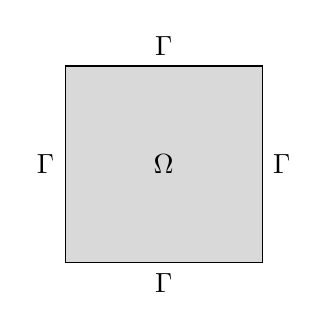
\begin{tikzpicture}[scale=2.5]
				% Draw the shaded square
				\fill[gray!30] (0,0) rectangle (1,1);
				
				% Draw the square outline
				\draw (0,0) rectangle (1,1);
				
				% Label Ω inside the square
				\node at (0.5,0.5) {$\Omega$};
				
				% Label Γ on the boundaries
				\node at (-0.1,0.5) {$\Gamma$};
				\node at (1.1,0.5) {$\Gamma$};
				\node at (0.5,-0.1) {$\Gamma$};
				\node at (0.5,1.1) {$\Gamma$};
			\end{tikzpicture}
			%\includegraphics[scale = 0.13]{images/domain.png}
			%\includegraphics[scale = 0.13]{images/domain_3d.png}
		\end{center}
	\end{column}
\end{columns}

\vspace{0.4cm}
\begin{itemize}
	\item This is an Advection-Diffusion problem for $T$. 
	\item The value of $\frac{1}{\epsilon}$ controls the Péclet number ($\mathrm{Pe}=\frac{1}{\epsilon}$).
	\item The higher the Péclet number is, the more hyperbolic the equation becomes.
\end{itemize}    

\visible<2->{
	\textcolor{UniBlue}{$\longrightarrow$ The next step is to discretize the equation using the \textbf{finite difference method}.}}
\end{frame}


\begin{frame}
	\frametitle{\textbf{1. Problem A: FDM}}
	
	\begin{columns}[c]
		\begin{column}{0.5\textwidth}
			% \vspace*{-\baselineskip}
			\begin{framed}
				Find a scalar $T$ in $\Omega \rightarrow \mathbb{R}$ satisfying:
				\begin{align*}
					\partial_j \partial_j T =& 1 \ \textrm{ in } \Omega\\
					T =& 0 \ \textrm{ in } \Gamma
				\end{align*}
			\end{framed}
		\end{column}
		\begin{column}{0.4\textwidth}
			\vspace*{-\baselineskip}
			\begin{center}
				
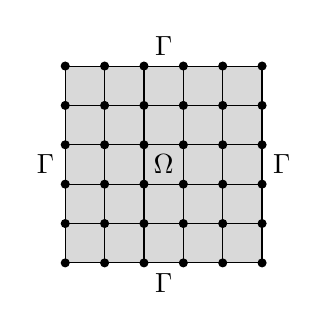
\begin{tikzpicture}[scale=2.5]
	% Draw the square outline
\fill[gray!30] (0,0) rectangle (1,1);
	
    
% Draw the grid lines inside the square
\foreach \x in {0.2,0.4,0.6,0.8}
\draw (\x,0) -- (\x,1);
\foreach \y in {0.2,0.4,0.6,0.8}
\draw (0,\y) -- (1,\y);

% Draw the grid lines outside the square
\draw (0,0) grid (1,1);

% Draw circles inside the square and in the corners
\foreach \x in {0.2,0.4,0.6,0.8}
\foreach \y in {0.2,0.4,0.6,0.8}
\filldraw (\x,\y) circle (0.02);
\foreach \x in {0,1}
\foreach \y in {0,1}
\filldraw (\x,\y) circle (0.02);

% Label Ω inside the square
\node at (0.5,0.5) {$\Omega$};

% Label Γ on the boundaries
\node at (-0.1,0.5) {$\Gamma$};
\node at (1.1,0.5) {$\Gamma$};
\node at (0.5,-0.1) {$\Gamma$};
\node at (0.5,1.1) {$\Gamma$};

% Draw nodes on the sides
\foreach \x in {0.2,0.4,0.6,0.8}
\filldraw (\x,0) circle (0.02);
\foreach \y in {0.2,0.4,0.6,0.8}
\filldraw (0,\y) circle (0.02);
\foreach \x in {0.2,0.4,0.6,0.8}
\filldraw (\x,1) circle (0.02);
\foreach \y in {0.2,0.4,0.6,0.8}
\filldraw (1,\y) circle (0.02);

\end{tikzpicture}
				%\includegraphics[scale = 0.13]{images/domain.png}
				%\includegraphics[scale = 0.13]{images/domain_3d.png}
			\end{center}
		\end{column}
	\end{columns}
	
	\vspace{0.4cm}
We divide the domain into a grid and obtain:
\begin{align*}
	\frac{1}{\Delta x^2} \pp{-T_{i+1} + 2T_{i} - T_{i-1}} + \frac{1}{\Delta y^2} \pp{-T_{i+n_x} + 2T_{i} - T_{i-n_x}} &= 1  \ \forall i \in \Omega
	\\
	T_i &= 0 \  \forall i \in \Gamma
\end{align*}  
\end{frame}

\begin{frame}
	\frametitle{\textbf{1. Problem B: FDM}}
	
	\begin{columns}[c]
		\begin{column}{0.5\textwidth}
			% \vspace*{-\baselineskip}
		\begin{framed}
	Find a scalar $T$ in $\Omega \rightarrow \mathbb{R}$ satisfying:
	\begin{align*}
		u_j \partial_j T + \epsilon \partial_j \partial_j T =& 1 \ \textrm{ in } \Omega\\
		T =& 0 \ \textrm{ in } \Gamma \\
		u_j =& 1 \ \forall j \in [1,d]
	\end{align*}
\end{framed}
		\end{column}
		\begin{column}{0.4\textwidth}
			\vspace*{-\baselineskip}
			\begin{center}
				
				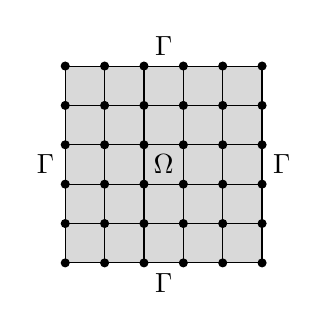
\begin{tikzpicture}[scale=2.5]
					% Draw the square outline
					\fill[gray!30] (0,0) rectangle (1,1);
					
					
					% Draw the grid lines inside the square
					\foreach \x in {0.2,0.4,0.6,0.8}
					\draw (\x,0) -- (\x,1);
					\foreach \y in {0.2,0.4,0.6,0.8}
					\draw (0,\y) -- (1,\y);
					
					% Draw the grid lines outside the square
					\draw (0,0) grid (1,1);
					
					% Draw circles inside the square and in the corners
					\foreach \x in {0.2,0.4,0.6,0.8}
					\foreach \y in {0.2,0.4,0.6,0.8}
					\filldraw (\x,\y) circle (0.02);
					\foreach \x in {0,1}
					\foreach \y in {0,1}
					\filldraw (\x,\y) circle (0.02);
					
					% Label Ω inside the square
					\node at (0.5,0.5) {$\Omega$};
					
					% Label Γ on the boundaries
					\node at (-0.1,0.5) {$\Gamma$};
					\node at (1.1,0.5) {$\Gamma$};
					\node at (0.5,-0.1) {$\Gamma$};
					\node at (0.5,1.1) {$\Gamma$};
					
					% Draw nodes on the sides
					\foreach \x in {0.2,0.4,0.6,0.8}
					\filldraw (\x,0) circle (0.02);
					\foreach \y in {0.2,0.4,0.6,0.8}
					\filldraw (0,\y) circle (0.02);
					\foreach \x in {0.2,0.4,0.6,0.8}
					\filldraw (\x,1) circle (0.02);
					\foreach \y in {0.2,0.4,0.6,0.8}
					\filldraw (1,\y) circle (0.02);
					
				\end{tikzpicture}
				%\includegraphics[scale = 0.13]{images/domain.png}
				%\includegraphics[scale = 0.13]{images/domain_3d.png}
			\end{center}
		\end{column}
	\end{columns}
	
	\vspace{0.4cm}
	We divide the domain into a grid and obtain:
	\begin{align*}
		&\frac{1}{\Delta x^2} \pp{(-1+\frac{u_x \Delta x}{2\epsilon})T_{i+1} + 2T_{i} + (-1-\frac{u_x \Delta x}{2\epsilon})T_{i-1}} +\\ &\frac{1}{\Delta y^2} \pp{(-1+\frac{u_y \Delta y}{2\epsilon})T_{i+n_x} + 2T_{i} + (-1-\frac{u_y\Delta y}{2\epsilon}) T_{i-n_x}} = 10  \ \forall i \in \Omega
		\\
		&T_i = 0 \  \forall i \in \Gamma
	\end{align*}  
\end{frame}


\pgfplotstableread{data2d.dat}\secondtable
\def\nrowsb{35}
\def\ncolsb{35}
\begin{frame}
	\frametitle{\textbf{1. Sparsity pattern of the matrix}}
	
The matrix A is penta-diagonal. For $n$ nodes it has a maximum of 5 non-zero elements. 

\begin{figure}
	%
	\centering
	\resizebox{0.65\linewidth}{!}{
		\begin{tikzpicture}
			\foreach \i in {0,...,\nrowsb}{
				\foreach \j in {0,...,\ncolsb}{
					\pgfplotstablegetelem{\i}{\j}\of\secondtable
					\ifnum\pgfplotsretval=0 \node[rectangle, rounded corners, minimum size=15pt, inner sep=5pt, fill=gray, opacity=0.2] at (\j*20 pt,-\i*20 pt) {}; \fi
					\ifnum\pgfplotsretval=1
					\node[rectangle, rounded corners, minimum size=15pt, inner sep=5pt, fill=gray!\pgfplotsretval!red, opacity=0.5*\pgfplotsretval] at (\j*20 pt,-\i*20 pt) {};
					\fi
					\ifnum\pgfplotsretval=2
					\node[rectangle, rounded corners, minimum size=15pt, inner sep=5pt, fill=gray!\pgfplotsretval!blue, opacity=0.25*\pgfplotsretval] at (\j*20 pt,-\i*20 pt) {};
					\fi
				};
			};
		\end{tikzpicture}
	}
	%		\caption{}
	%		\label{}
\end{figure}
\end{frame}


\begin{frame}[fragile]
	\frametitle{\textbf{1. Problem A: Python code part 1}}


\begin{PYTHON}
def fill_matrix_poisson(A,b,nx,ny):
  N = nx*ny
  dx = 1./ (nx-1)
  dy = 1./ (ny-1)
  Sx = 1 / dx**2
  Sy = 1 / dy**2
  
  # Boundary conditions bottom
  for i in range(0,nx):
    A[i,i] = 1
    b[i] = 0
  
  # Boundary condition top
  for i in range(0,nx):
    k = (ny-1)*nx+i
    A[k,k] = 1
    b[k] = 0
  
  # Boundary condition left
  for j in range(0,ny):
    k = nx*(j)
    A[k,k] = 1
    b[k] = 0

\end{PYTHON}

\end{frame}

\begin{frame}[fragile]
	\frametitle{\textbf{1. Problem A: Python code part 2}}
	
	
	\begin{PYTHON}

# Boundary condition right
for j in range(0,ny):
  k = (nx-1)+nx*(j-1)
  A[k,k] = 1
  b[k] = 0      

# Inside
for i in range(1,nx-1):
  for j in range(1,ny-1):
    k = i+nx*j
    A[k,k-nx] = -Sy
    A[k,k-1] = -Sx
    A[k,k] = (2*Sx+2*Sy)
    A[k,k+1] = -Sx
    A[k,k+nx] = -Sy
    b[k] = 10
\end{PYTHON}
	
\end{frame}

